
\documentclass{report}
\usepackage{amssymb, amsmath}
\usepackage{graphicx}
\usepackage{float}

\title{Reporte Tarea 4}
\date{12 de Octubre de 2022}
\author{Nestor Adrian Sandoval Ortiz}

\begin{document}
    \maketitle

    \chapter{Funciones monovariables}
        \paragraph{Introduccion}
        A continuacion se presentan 5 funciones que serviran como punto de comparacion para 5 algoritmos de optimizacion sin restricciones.
        Es importante mencionar que, con el fin de mantener una condicion y/o cantidad de iteraciones justa, se ha planteado al numero "100"
        como parametro de "paro" en todas las funciones, es decir, en aquellas funciones que dependan de un determinado numero de iteraciones,
        estas sumaran 100, mientras que, en las que dependan de un valor concreto de "error", este mismo sera ubicado de tal forma que sus cantidades
        de iteraciones sean lo mas cercanas a 100
        Por ultimo, cabe destacar que se realizaran 1000 ejecuciones independientes de cada algoritmo, con el fin de conocer la media de sus valores
        asi como su mejor y peor desempeño.

        \pagebreak

        \section{Primera Funcion}
            \begin{equation*}
                f(x)=3x^4+(x-1)^2
            \end{equation*}

            \begin{figure}[H]
                \includegraphics[width=\linewidth]{/Users/lloydna/Desktop/UP/5° Semestre/Optimizacion/Optimizacion/Tareas/Tarea4/Parte1/Ejercicio1/Funcion.png}
                \caption{Grafica de la funcion}
                \label{fig:fun11}
            \end{figure}

            \subsection{Tabla de resultados}
                \begin{tabular}{l|c|c|c|c|c|c}
                    & x Promedio & f(x) Promedio & Mejor x & Mejor f(x) & Peor x & Peor f(x)\\
                    \hline
                    Ajuste Polinomial Cubico & 0.45131 & 0.42552 & 0.45131 & 0.42552 & 0.45131 & 0.42552\\
                    \hline
                    Biseccion & 0.4375 & 0.42632 & 0.4375 & 0.42632 & 0.4375 & 0.42632\\
                    \hline
                    Gradiente & 0.4507 & 0.42552 & 0.4507 & 0.42552 & 0.4507 & 0.42552\\
                    \hline
                    Newton Raphson & 0.45071 & 0.42552 & 0.45071 & 0.42552 & 0.45071 & 0.42552\\
                    \hline
                    Secante & 0.45059 & 0.42552 & 0.45059 & 0.42552 & 0.45059 & 0.42552\\
                    \hline
                \end{tabular}
        \pagebreak

        \section{Segunda Funcion}
            \begin{equation*}
                f(x)=-4xsin(x)
            \end{equation*}

            \begin{figure}[H]
                \includegraphics[width=\linewidth]{/Users/lloydna/Desktop/UP/5° Semestre/Optimizacion/Optimizacion/Tareas/Tarea4/Parte1/Ejercicio2/Funcion.png}
                \caption{Grafica de la funcion}
                \label{fig:fun12}
            \end{figure}

            \subsection{Tabla de resultados}
            \begin{tabular}{l|c|c|c|c|c|c}
                & x Promedio & f(x) Promedio & Mejor x & Mejor f(x) & Peor x & Peor f(x)\\
                \hline
                Ajuste Polinomial Cubico & 2.03057 & -7.27881 & 2.03057 & -7.27881 & 2.03057 & -7.27881\\
                \hline
                Biseccion & 2.001 & -7.27468 & 2.001 & -7.27468 & 2.001 & -7.27468\\
                \hline
                Gradiente & 2.02876 & -7.27882 & 2.02876 & -7.27882 & 2.02876 & -7.27882\\
                \hline
                Newton Raphson & 2.02886 & -7.27882 & 2.02886 & -7.27882 & 2.02886 & -7.27882\\
                \hline
                Secante & 2.0284 & -7.27882 & 2.0284 & -7.27882 & 2.0284 & -7.27882\\
                \hline
            \end{tabular}
        \pagebreak

        \section{Tercera Funcion}
            \begin{equation*}
                f(x)=2(x-3)^2+exp(0.5x^2)
            \end{equation*}

            \begin{figure}[H]
                \includegraphics[width=\linewidth]{/Users/lloydna/Desktop/UP/5° Semestre/Optimizacion/Optimizacion/Tareas/Tarea4/Parte1/Ejercicio3/Funcion.png}
                \caption{Grafica de la funcion}
                \label{fig:fun13}
            \end{figure}

            \subsection{Tabla de resultados}
            \begin{tabular}{l|c|c|c|c|c|c}
                & x Promedio & f(x) Promedio & Mejor x & Mejor f(x) & Peor x & Peor f(x)\\
                \hline
                Ajuste Polinomial Cubico & 1.59368 & 7.516 & 1.59368 & 7.516 & 1.59368 & 7.516\\
                \hline
                Biseccion & 1.5625 & 7.52238 & 1.5625 & 7.52238 & 1.5625 & 7.52238\\
                \hline
                Gradiente & 1.59072 & 7.51592 & 1.59072 & 7.51592 & 1.59072 & 7.51592\\
                \hline
                Newton Raphson & 1.59373 & 7.516 & 1.59373 & 7.516 & 1.59373 & 7.516\\
                \hline
                Secante & 1.58894 & 7.51595 & 1.58894 & 7.51595 & 1.58894 & 7.51595\\
                \hline
            \end{tabular}
        \pagebreak

        \section{Cuarta Funcion}
            \begin{equation*}
                f(x)=3x^2+12/x^3-5
            \end{equation*}

            \begin{figure}[H]
                \includegraphics[width=\linewidth]{/Users/lloydna/Desktop/UP/5° Semestre/Optimizacion/Optimizacion/Tareas/Tarea4/Parte1/Ejercicio4/Funcion.png}
                \caption{Grafica de la funcion}
                \label{fig:fun14}
            \end{figure}

            \subsection{Tabla de resultados}
            \begin{tabular}{l|c|c|c|c|c|c}
                & x Promedio & f(x) Promedio & Mejor x & Mejor f(x) & Peor x & Peor f(x)\\
                \hline
                Ajuste Polinomial Cubico & 1.43144 & 5.23837 & 1.43144 & 5.23837 & 1.43144 & 5.23837\\
                \hline
                Biseccion & 1.40625 & 5.24774 & 1.40625 & 5.24774 & 1.40625 & 5.24774\\
                \hline
                Gradiente & 1.43097 & 5.23836 & 1.43097 & 5.23836 & 1.43097 & 5.23836\\
                \hline
                Newton Raphson & 1.43091 & 5.23836 & 1.43091 & 5.23836 & 1.43091 & 5.23836\\
                \hline
                Secante & 1.43264 & 5.2384 & 1.43264 & 5.2384 & 1.43264 & 5.2384\\
                \hline
            \end{tabular}
        \pagebreak

        \section{Quinta Funcion}
            \begin{equation*}
                f(x)=2x^2+16/x
            \end{equation*}

            \begin{figure}[H]
                \includegraphics[width=\linewidth]{/Users/lloydna/Desktop/UP/5° Semestre/Optimizacion/Optimizacion/Tareas/Tarea4/Parte1/Ejercicio5/Funcion.png}
                \caption{Grafica de la funcion}
                \label{fig:fun15}
            \end{figure}

            \subsection{Tabla de resultados}
            \begin{tabular}{l|c|c|c|c|c|c}
                & x Promedio & f(x) Promedio & Mejor x & Mejor f(x) & Peor x & Peor f(x)\\
                \hline
                Ajuste Polinomial Cubico & 1.58744 & 15.11905 & 1.58744 & 15.11905 & 1.58744 & 15.11905\\
                \hline
                Biseccion & 1.5625 & 15.12281 & 1.5625 & 15.12281 & 1.5625 & 15.12281\\
                \hline
                Gradiente & 1.5874 & 15.11905 & 1.5874 & 15.11905 & 1.5874 & 15.11905\\
                \hline
                Newton Raphson & 1.58657 & 15.11906 & 1.58657 & 15.11906 & 1.58657 & 15.11906\\
                \hline
                Secante & 1.58962 & 15.11908 & 1.58962 & 15.11908 & 1.58962 & 15.11908\\
                \hline
            \end{tabular}
        \pagebreak

        \section{Analisis de resultados}

    \chapter{Funciones multivariables}
        \paragraph{Introduccion}
        Introduccion aqui

        \section{Primera Funcion}
            \subsection{Tabla de resultados}
            \subsection{Analisis de resultados}

        \section{Segunda Funcion}
            \subsection{Tabla de resultados}
            \subsection{Analisis de resultados}

        \section{Tercera Funcion}
            \subsection{Tabla de resultados}
            \subsection{Analisis de resultados}

        \section{Cuarta Funcion}
            \subsection{Tabla de resultados}
            \subsection{Analisis de resultados}

        \section{Quinta Funcion}
            \subsection{Tabla de resultados}
            \subsection{Analisis de resultados} 
\end{document}